\documentclass{beamer}

% Top-aligning columns within a top-aligned frame
% https://tex.stackexchange.com/questions/16447/beamer-top-aligning-columns-within-a-top-aligned-frame
\makeatletter
\newenvironment{myitemize}{%
   \setlength{\topsep}{0pt}
   \setlength{\partopsep}{0pt}
   \renewcommand*{\@listi}{\leftmargin\leftmargini \parsep\z@ \topsep\z@ \itemsep\z@}
   \let\@listI\@listi
   \itemize
}{\enditemize}
\makeatother  

\usepackage[USenglish]{babel}
\usepackage[utf8]{inputenc}
\usepackage{amssymb, amsmath}
\usepackage{bm}
\usepackage{color}
\usepackage{tikz}
\usepackage{url}

\definecolor{links}{HTML}{2A1B81}
\hypersetup{colorlinks,linkcolor=,urlcolor=links}

\usetheme{Boadilla}
\setbeamertemplate{headline}{}
\newcommand*\oldmacro{}%
\let\oldmacro\insertshorttitle%
\renewcommand*\insertshorttitle{%
  \oldmacro\hfill%
  \insertframenumber\,/\,\inserttotalframenumber}
  

\bibliographystyle{apalike}
% make bibliography entries smaller
%\renewcommand\bibfont{\scriptsize}
% Now get rid of all the colours
\setbeamercolor*{bibliography entry title}{fg=black}
\setbeamercolor*{bibliography entry author}{fg=black}
\setbeamercolor*{bibliography entry location}{fg=black}
\setbeamercolor*{bibliography entry note}{fg=black}

\newcommand{\lnorm}[1]{\left\lVert#1\right\rVert^2}
\newcommand{\norm}[1]{\left\lVert#1\right\rVert}

% and kill the abominable icon
\setbeamertemplate{bibliography item}{}

\begin{document}
\title{HOP-Rec: High-Order Proximity for Implicit Recommendation}  
\author{Radek Bartyzal}
\date{18. 10. 2018} 
\institute{Let's talk ML in Prague}

\frame{\titlepage} 

\begin{frame}{Recommender systems}

\begin{figure}[h!]
\centering
\[
R = 
\begin{pmatrix}
    r_{11} & r_{12} & r_{13} & \dots  & r_{1m} \\
    r_{21} & r_{22} & r_{23} & \dots  & r_{2m} \\
    \vdots & \vdots & \vdots & \ddots & \vdots \\
    r_{n1} & r_{n2} & r_{n3} & \dots  & r_{nm}
\end{pmatrix}
\]
\caption{User-item matrix of rating values.}
\label{fig:rating-matrix}
\end{figure}

Recommendation algorithm types:
\begin{itemize}
\item Factorization based
\item Graph based
\item Other
\end{itemize}

\end{frame}
%--------- END Frame 1 -------------

\begin{frame}{Algorithm types}

\begin{itemize}
\item \textbf{Factorization based:} Get lower dimensional vector representation (embedding) of each user and each item. Then use these embeddings as an input to other recommendation algorithms.\vfill

\item \textbf{Graph based:} Construct a bipartite graph from the rating matrix. Ratings are edge weights. Traverse graph in certain ways to get user preferences.
\end{itemize}

\end{frame}
%--------- END Frame 2 -------------

\begin{frame}{Matrix factorization}

\begin{figure}[h]
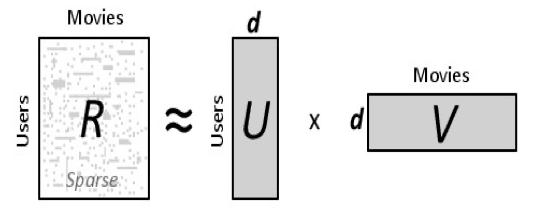
\includegraphics[scale=0.60]{img/matrix_factorization}
\end{figure}


$$
Loss = \lnorm{R - UV^T} + \lambda \lnorm{U} + \lambda \lnorm{V} 
$$

\end{frame}
%--------- END Frame 3 -------------

\begin{frame}{HOP-Rec}

\begin{itemize}
\item combine factorized with graph based
\item use implicit ratings = 1 or unknown
\end{itemize}

\end{frame}
%--------- END Frame 4 -------------
\begin{frame}{HOP-Rec}

Graph: 
\begin{itemize}
\item nodes = users  $\cup$ items
\item edges = known implicit ratings, no weights
\end{itemize}

Random walk through graph:
\begin{enumerate}
\item start at user $u$ = $u_0$
\item go through $k-1$ items and $k-1$ users to end at item $i_k$
\item resulting sequence $S = (u_0, i_1, u_1, \cdots , i_{k-1}, u_{k-1}, i_{k})$
\item K typically low = 1 - 3
\end{enumerate}

\end{frame}
%--------- END Frame 4 -------------
\begin{frame}{HOP-Rec}

\begin{figure}[h]
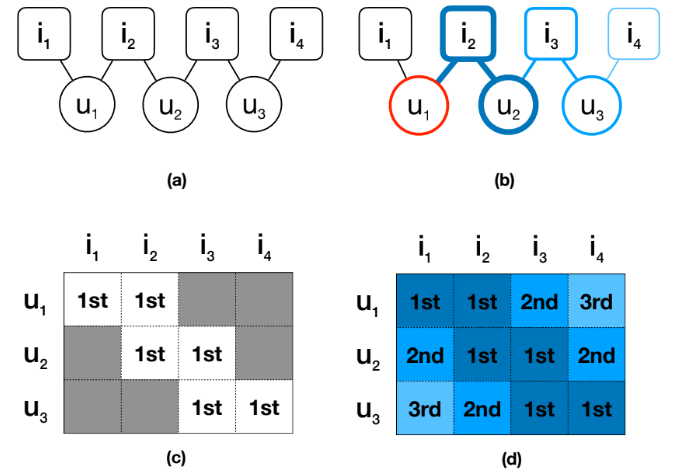
\includegraphics[scale=0.60]{img/hop-rec}
\caption{High-order proximity between users and items
within observed interactions \cite{cit:hop-rec}.}
\end{figure}

\end{frame}
%--------- END Frame 5 -------------
\begin{frame}{HOP-Rec}

\begin{figure}[h]
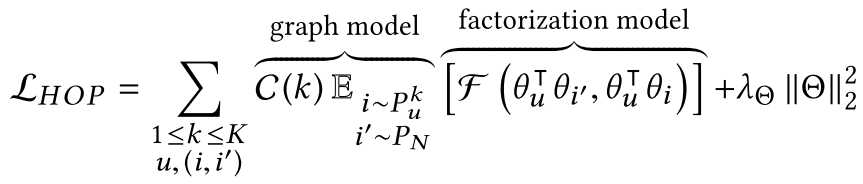
\includegraphics[scale=0.60]{img/loss}
\end{figure}

$P_u^k$ = k-order probability distribution for an
item sampled from Su

$P_N$ = uniform distribution over all items = $i'$ is random item

$C(k) = \frac{1}{k}$ = weight = how close is the item to the user in graph

\begin{figure}[h]
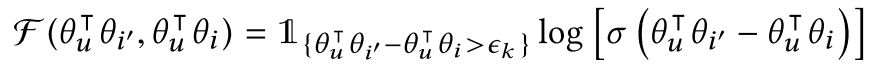
\includegraphics[scale=0.60]{img/log-loss}
\caption{Ranking loss = indicator * pairwise logistic loss \cite{cit:hop-rec}.}
\end{figure}

Indicator = if predicted rating of random item is higher than for the known item, then optimize their embeddings to change that

\end{frame}
%--------- END Frame 6 -------------
\begin{frame}{Training}

\begin{enumerate}
\item Do this for each user $u$:
\item sample item $i$ from random walk
\item sample random item $i'$
\item optimize embeddings of $u$, $i$, $i'$ by Asynchronous SGD to predict higher rating for $(u,i)$ than for $(u,i')$ 
\end{enumerate}
\vfill
\textbf{Whats the point?}

Instead of giving SGD just the known ratings and then all the rest as unknown we increase the number of 'known' examples by selecting higher-order neighbor items and present them to SGD with lower weight than the original first-order known ratings.

\end{frame}
%--------- END Frame 7 -------------
\begin{frame}{Results}

\end{frame}
%--------- END Frame 7 -------------


%--------- END Frame 12 -------------
\begin{frame}{Sources}

\begin{thebibliography}{0}

  \bibitem[1]{cit:hop-rec} 1. Yang, Jheng-Hong, et al. "HOP-rec: high-order proximity for implicit recommendation." Proceedings of the 12th ACM Conference on Recommender Systems. ACM, 2018.
  
\end{thebibliography}

\end{frame}

 
 
 
\end{document}
